%\section{Mathematical Modeling}
\label{sec:mathmodel}

% \begin{itemize}
% \item \st{unstable stratified boundary layers (raleigh number estimate)}
% \item \st{justify incompressible N-S}
% \item \st{justification of far-field eddy-viscosity model (M-O)}
% \item modeling eddy-viscosity in device 
% \item vane and turbine representation via penalty function // immersed boundary method
% \item cone representation
% \end{itemize}

%remember that \st{} is strikethrough
%
% should this all be math modeling?
%

The aim of this work is to simulate synthetic
dust devils in the field. This requires a model of the ambient
conditions for a representative case, such as Arizona, where
experimental data is available from tests that have been
performed. Furthermore, for this to be generally useful in the
prediction of flows in a variety of conditions, we need a model
applicable to any flow near the surface of the earth.  

This chapter details an analysis of surface fluid mechanics, and
develops a mathematical model for turbulence in a thermally stratified
medium. We seek to emulate the operation of the apparatus during the
day, when dust devils are observed to form readily. 
At these times, the atmospheric surface layer has the following
character. Incident radiation from the Sun does not significantly
interact with the air, which is nearly
transparent\cite{haltiner1957dynamical}. Instead, this radiation is
absorbed by the ground, which causes its temperature to rise. This
results in a temperature difference between the hot ground and the cooler
air. The ground heats the air, causing expansion and lowering the density
of the air. This reduced density air near the surface is then driven
upwards by buoyancy.    

For sufficiently large temperature differences, the hot surface layer is
unstable, and as the warm air is driven upwards the flow will transition
to turbulence. For the typical use case we consider, namely Arizona in
summer, the temperature difference can be in excess of 30 Kelvin. 
Rayleigh numbers associated with temperature differences of this
magnitude are between $10^{9} - 10^{11}$ and therefore meets the
criterion\cite{incropera1996fundamentals}  
for transition to a turbulent regime. The flow is that of an unstably
stratified fluid.  

This chapter begins by describing the governing equations of the system
of interest. It then proceeds to the development of a viscosity model
used to resolve the large scale features of the solution. Next, models
used to represent the vanes and turbine, are introduced.  Finally, the
models for the computational domain extent and the boundary conditions
are discussed. 

%Note that a complete numerical specification of all the model
%parameters introduced in this chapter are provided in a table in
%appendix \ref{app:model_param}.

\section{The Governing Equations of Fluid Motion}
\label{sub_sec:ns_en}

The equations describing fluid flow with natural convection are,
\begin{align}
  \frac{\partial {\bf u}}{\partial t} + {\bf u} \cdot \nabla {\bf u} =& \,
  -\frac{1}{\rho}\nabla P + \nu \nabla^2 {\bf u} - {\bf g} \frac{T'}{T_0}
 \label{eq:ns} \\
  \nabla \cdot {\bf u} =& \, 0 \label{eq:cont} \\
  \rho c_p \frac{\partial T}{\partial t} + {\bf u} \cdot \nabla T =& \, \nabla
 \cdot ( k \nabla T) \label{eq:ht}
\end{align} 
under the assumption that the temperature variation is small in
comparison to the mean temperature of the region. These are the
incompressible Navier-Stokes equations with the Boussinesq
approximation\cite{boussinesq2010théorie}, a representation of buoyancy
coupled with the heat equation. Note that in
Equations~\ref{eq:ns}-\ref{eq:ht}, and throughout this document,
boldface denotes a vector quantity, for example, ${\bf u} = \{u,v,w\}$.  
Furthermore, these equations ignore the action of the Coriolis force. 
Monin and Obukhov~\cite{monin1954basic} demonstrated that the Coriolis
force is negligible for the surface layer below fifty meters (a distance
well below our region of interest), and this argument is detailed in
Appendix~\ref{appendix:coriolis}.  

As discussed above, we anticipate that the flow will be sufficiently
high Reynolds number as to be
turbulent~\cite{Reynolds01011883}. Turbulence significantly alters the
character of the flow,  
and necessitates either resolving the resulting small scales or
providing a model that represents their impact. In this case, 
%a Reynolds Averaged Navier-Stokes (RANS) formulation is used, where 
the turbulent viscosity and thermal conductivities are permitted to vary in
space, and the flow is decomposed into constant laminar
($\nu_{l},K_{l}$), varying turbulent ($\nu_{t},K_{t}$), and vane
($\nu_{V},K_{V}$) components, 

\begin{eqnarray}
 \nu =& \nu_{l} + \nu_{t}(z) + \nu_{V}(r,z), \label{eqn:visc_tot}\\
 K =& K_{l} + K_{t}(z) + K_{V}(r,z). \label{eqn:therm_tot}
\end{eqnarray}

This is an effective eddy viscosity model\cite{boussinesq1887}, and the
subsequent two sections will elaborate on the spatial dependence and
character of $\nu_t$, $K_t$, $\nu_V$ and $K_V$. The laminar, base
diffusivities are $\nu_l$ and $K_l$, and do not vary in space.  

\section{Viscosity Model}

We use the well-known similarity model of Monin and
Obukhov\cite{monin2007statistical,1990JFM...212..637K} as
a guide to the specification of an eddy viscosity model to describe the
vertical mixing in the atmosphere.
This formulation is an extension of
the mixing-length model of Prandtl, where the concepts of gradient
diffusion and mixing length were generalized to thermally stratified
flow. This section details the Monin-Obukhov scaling through the lens 
of dimensional analysis. 

%ADD DIMENSIONS TO MAKE SCALING MORE CLEAR\todo{add dimensions}
%
% justify prandtl assumption here
%

Monin and Obukhov argued that under statistically stationary, horizontally
homogeneous conditions, the dynamics of any mean turbulent quantity
($\bar f$) in a thermally stratified medium depend only on,  

\begin{equation}
%\bar f = f(z,\frac{g}{T_0},\rho_0,\nu_l,K_l,u^*,q,c_p).
\bar f = f(z,\frac{g}{T_0},\nu_l,K_l,u^*,\rho_0,\frac{q}{\rho_0 \, c_p}).
\end{equation}
Aside from near the surface, the laminar diffusivities $\nu_l$ 
and $K_l$ will be  
small compared to their turbulent counterparts, $\nu_t$ and $K_t$, and 
are therefore negligible. 
The remaining parameters are: the distance from the ground, z; the
buoyancy coefficient, $\frac{g}{T_0}$; 
the density of the fluid, $\rho_0$; 
a velocity scale, $u^*$ (in particular, the freestream
velocity); and the turbulent heat flux to the ground, $\frac{q}{\rho_0 c_p}$. 
%and the specific heat,
%$c_p$. %\todo{is this right?} 
% Likewise, if we define $z-z_0$ as an ``effective roughness
% height'' or displacement distance, we can reasonably neglect $z_0$ from these
% considerations. While the roughness height can be large (for instance in
% a cornfield, where the roughness height could reasonably be several
% meters), for the present study the expectation is that this roughness
% height will be on the order of centimeters\cite{oke1987boundary}, and
% therefore negligible.  
%
% add refence to dynamical and physical meteorology 
% 
These primary quantities have the following dimensions,

\begin{eqnarray}
 \textbf{Height:}& z\enskip \dot = \enskip [m]  \\
 \textbf{Buoyancy:}& \qquad \frac{g}{T_0}\enskip \dot = \enskip [kg] [m] [s]^{-2}
  [K]^{-1} \\ 
 \textbf{Velocity:}& \enskip u^* \enskip \dot = \enskip [m] [s]^{-1} \\
  \textbf{Density:}&  \enskip \rho_0 \enskip \dot = \enskip [kg] [m]^{-3}  \\
 \textbf{Heat Flux:}& \enskip \frac{q}{\rho_0 c_p} \enskip \dot = \enskip [K] [m]^{-1} [s]^{-1} \\
 % \textbf{Heat Flux:}& \enskip q \enskip \dot = \enskip [kg] [s]^{-3} \\
 % \textbf{Specific Heat:}& \enskip c_p \enskip \dot = \enskip [m]^2 [s]^{-2} [K]^{-1} 
\end{eqnarray}

The unknown mean turbulent quantity ($\bar f$) depends on four
dimensions: length, time, temperature and mass. Dimensional analysis
implies that this should then only be a function of a single dimensionless
group\cite{munson2012fundamentals}. This is chosen to be,
\begin{equation}
 \xi = -\frac{\kappa \frac{g}{T_0} \frac{q}{c_p \rho_0} z}{ {u^*}^3}.
\end{equation}
where $\kappa$ is the (dimensionless) Von-Karman constant. 
The physical meaning of this quantity bears some discussion.  
The numerator, $\kappa \frac{g}{T_0} \frac{q}{c_p \rho_0} $, is
proportional to the buoyant production of kinetic energy.  The
denominator, $\frac{{u^*}^3}{z}$, is a shear production rate. 
%
The non-dimensional group $\xi$ is typically cast into the following 
form, 
\begin{equation}
 \xi = \frac{z}{L_{M-O}},
\end{equation}
where $L_{M-O}$ is the famous, ``Monin-Obukhov'' length,
\begin{equation}
 L_{M-O} = -\frac{{u^*}^3}{\kappa \frac{g}{T_0} \frac{q}{c_p \rho_0}}. 
  \label{eqn_mo_length}
\end{equation}
%
This length can be interpreted as the vertical location
where the production of buoyantly generated kinetic energy is
approximately equal to the energy generated by wind shear. When the
magnitude of $L_{M-O}$ is large, the flow is dominated by shear effects,
and the impact of buoyancy is small. Conversely, a small magnitude of
$L_{M-O}$ implies that buoyant effects largely dominate the kinetic
energy production. Notice also that the sign convention in Equation
\ref{eqn_mo_length} is such that for the systems we consider ($q > 0$, heat
flux from the surface to the air), $L_{M-O}$ will always be
negative. This is as expected, as the convection from the high
temperature surface to cooler air is unstable. 
The scenarios considered in this document are for $\xi<0$, which
corresponds to heat flux from the ground into the air. 

%The mean quantity $\bar f$ has a
%functional representation to the effect,
The results of the scaling analysis imply that appropriately normalized
mean turbulent quantities should be functions only of a single 
non-dimensional group, 
\begin{equation}
 \frac{\bar f}{f_{MO}} = \phi(\frac{z}{L_{M-O}}), 
\end{equation}
where $f_{MO}$ is a normalizing constant with units of $\bar f$, and
$\phi$ is a function only of $\xi$. 
Monin-Obuhkov similarity theory has been shown to apply to a wide variety of
quantities\cite{wyngaard2010turbulence}, but we consider the velocity 
and temperature fields here. For instance, the mean velocity field would
have scaling, $\frac{u^*}{\kappa}$ and the temperature fields would be
scaled as $T^* = \frac{1}{\kappa u^*} \frac{q}{c_p \rho_0}$. In this
way, the mean velocity and temperature fields would have the form,  
\begin{eqnarray}
\bar u(z) = \frac{u^*}{\kappa} \phi_u(\frac{z}{L_{M-O}}), \\
\bar T(z) = T^* \phi_T(\frac{z}{L_{M-O}}).
\end{eqnarray}
Taking the derivative of these equations results in the mean 
vertical gradients of the velocity and temperature, which are,
\begin{eqnarray}
\frac{\partial \bar u(z)}{\partial z} = \frac{u^*}{\kappa \, L_{M-O}}
 \varphi_u(\frac{z}{L_{M-O}}) \label{eq:uz}, \\ 
\frac{\partial \bar T(z)}{\partial z} = \frac{T^*}{L_{M-O}}
 \varphi_T(\frac{z}{L_{M-O}}) \label{eq:tz}.
\end{eqnarray}
Where $\phi$ and $\varphi$ are different (and unknown) universal functions. Eddy
viscosity is defined as, $u'v' = \nu_t \frac{\partial
u}{\partial z}$\cite{durbin2001statistical}, in which case, using
equation \ref{eq:uz}, it can be expressed as, 
\begin{equation}
 \nu_t = \frac{{u^*}^2}{\frac{\partial \bar u}{\partial z}} = \frac{u^* \,
  \kappa \, L_{M-O}}{\varphi_u(\xi)}.
\end{equation}
While the eddy thermal diffusivity (defined as, $q = c_p \rho_0 K_T
\frac{\partial T}{\partial z}$) is,
\begin{equation}
 K_t = \frac{q/c_p \rho_0}{\frac{\partial \bar T}{\partial z}} = \frac{u^* \,
  \kappa \, L_{M-O}}{\varphi_T(\xi)}.
\label{eqn:eddy_kt}
\end{equation}
Note that while we have not assumed that $\varphi_u$ and
$\varphi_T$ are identical, for turbulent Prandtl numbers of unity 
(e.g. $Pr_t = 1$), they will be. We now consider the asymptotic behavior
of $\varphi_T$ and $\varphi_u$ at large and small values of $\xi$
to provides guidance as to the more general character of the functions. 

%Our interest lies in the case where $L_{M-O} \leq 0$, which corresponds
%to heat flux from the ground into the air.  
%

\subsection*{Case One: $\xi \to 0$}
The first case is the limit
%, is equivalent to the scenario where
%$\frac{z}{L_{M-O}} \to 0$, or 
$L_{M-O}>>z$, $\xi \to 0$. This occurs as the heat flux
at the wall approaches zero (e.g. $q \to 0$). 
This is purely wind driven flow with no thermal variation. 
In this limit, the profile is expected to be the ``log-law''. 
Equation~\ref{eq:uz} can be rearranged to obtain, 
%\begin{equation}
% \frac{\partial \bar u(z)}{\partial z} = \frac{u^*}{\kappa L_{M-O}} \varphi_u(\frac{z}{L_{M-O}}).
%\end{equation}
%After substituting $L_{M-O}=\frac{z}{\xi}$, 
\begin{equation}
 \frac{\partial \bar u(z)}{\partial z} = \frac{u^*}{\kappa z} \xi \varphi_u(\xi).
\end{equation}
%This is clearer if the substitution, $\Phi(\xi) = \xi \, \varphi(\xi)$, is made,
%\begin{equation}
% \frac{\partial \bar u(z)}{\partial z} = \frac{u^*}{\kappa z} \Phi(\xi).
%\end{equation}
In the log-layer, 
\begin{equation}
 \frac{\partial \bar u(z)}{\partial z} = \frac{u^*}{\kappa z},
\end{equation}
if $u^*$ is the friction velocity, $u_{\tau}$. 
%One can now more easily see that this function results in a logarithmic
%profile when $\Phi(\xi) = 1$, which in turn implies that for 
Therefore, for neutral stratification $(\xi = 0)$, 
\begin{equation}
 \lim_{\xi \to 0} \, \xi \, \varphi(\xi)= 1. 
\end{equation}
%We expect this to be approximately true for all small values of
%$\xi$, e.g. 
When $ |\frac{z}{L_{M-O}}| << 1$ it is therefore expected that,
\begin{equation}
 \varphi_u(\xi) \approx \text{ln } \rvert \frac{z}{L_{M-O}} \rvert + C.
\end{equation}
Identical arguments can be made for the asymptotic 
behaviour of the temperature function.

\subsection*{Case Two: $\xi \to -\infty$}

The case where $\xi \to -\infty $ implies $z>>L_{M-O}$.  
This is most readily interpreted as the instance
where $u^* \to 0$, e.g. the buoyancy-dominated case with no wind
(free-convection). This condition is typically referred to as,
``Thermal-only'' in this text. 
% hacking
%
For Equation~\ref{eq:tz} to be non-trivial (and
non-singular) in the limit as $\xi \to -\infty$, it must have no
dependence on $u^*$. A glance at this equation shows that
$T^* \thicksim \frac{1}{u^*}$, and $L \thicksim
{u^*}^{3}$. The non-dimensional scale, $\xi$, includes a
$(u^*)^{-3}$ factor through the dependence on the M-O length, 
$L_{M-O}$, in the denominator. 
Therefore, the overall function will not depend on $u^*$ only when
the function $\varphi$ is proportional to  $\xi^{-\frac{4}{3}}$. 

This means that the gradient in temperature has the following form,
\begin{equation}
\frac{\partial \bar T(z)}{\partial z} = -C_T \left(\frac{q}{c_p \,
					      \rho_0}\right)^\frac{2}{3}
\left( \frac{g}{T_0} \right)^{-\frac{1}{3}} z^{-\frac{4}{3}}  \text{
for } z \gg L.
\end{equation}

Where $C_T$ is some unknown multiplicative scaling constant. 
% hacking ends
Using this information in Equation~\ref{eqn:eddy_kt} provides an
expression for the asymptotic behavior of the thermal diffusivity, 
\begin{equation}
 K_t = -\frac{q}{c_p \, \rho_0 \, \frac{\partial \bar T(z)}{\partial z}}
  = \frac{1}{C_T} \left( \frac{q}{c_p \rho_0} \frac{g}{T_0}
		     \right)^\frac{1}{3} z^{\frac{4}{3}}  \text{ 
for } z \gg L_{M-O}. 
\end{equation}

So long as the turbulent Prandtl number remains constant in space, a
reasonable assumption~\cite{chuang1969turbulent}, then 
identical arguments regarding the asymptotic behaviour at large $\xi$
provide the analogous result for the eddy viscosity's variation with
respect to distance from the ground,   
\begin{equation}
 \nu_t = \frac{1}{C_{\nu_t}} \left( \frac{q}{c_p \rho_0} \frac{g}{T_0}
			     \right)^\frac{1}{3} z^{\frac{4}{3}}  \text{ 
for } z \gg L_{M-O}. 
\end{equation}


\subsection*{Approximations of the Universal Function}

We have now derived two criterion that our desired function of $\xi$ 
must capture. Namely, that for small values of negative $\xi$, the
function should be nearly identical to the logarithmic profiles
associated with neutral stratification. Secondly, at large negative
values of $\xi$, the function should go to
$\xi^{-\frac{4}{3}}$. Finally, the function should smoothly vary between
these conditions.  

There are several different functions, which are essentially different
calibrations of the same underlying function for different regimes with 
varying relative merits. 
Most functions are formulated in terms of $\Phi(\xi)$, 
not $\varphi(\xi)$. As
$\varphi(\xi) \thicksim \xi^{-\frac{4}{3}}$, and recalling that
$\Phi(\xi) = \xi \, \varphi(\xi)$, we expect 
$\Phi(\xi)$ to scale as $\xi^{-\frac{1}{3}}$.
%
%\cite{?}.\todo{missing cites} 
However, the functions are generally in close agreement under neutral
and unstable conditions, with the disagreement primarily occuring for
$z/L>0$. As we expect to only simulate conditions of unstable or
neutrally stratified flow, our choice of interpolation function does not
have a significant impact on the predicted value.  

\begin{figure}[!htb]
 \centering
  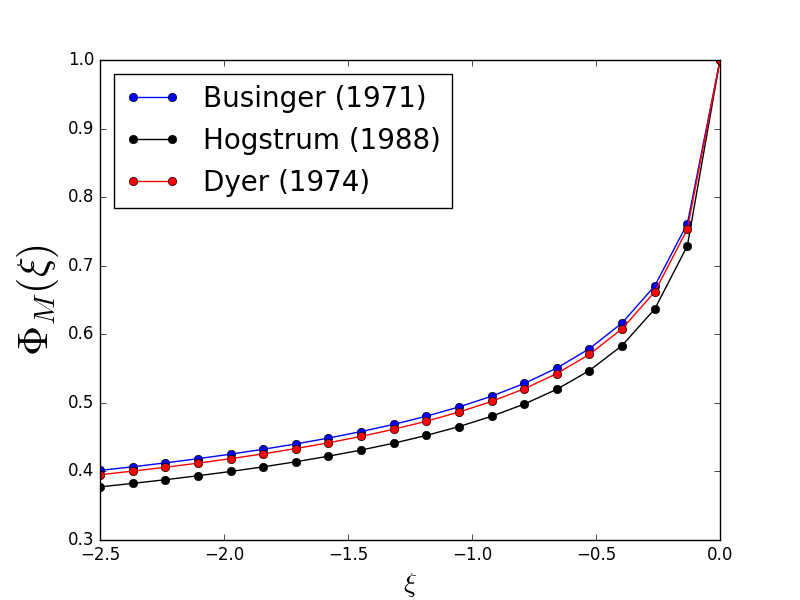
\includegraphics[width=.7\linewidth]{figs/mo-compare}\\
 \caption{Comparison between three common interpolation functions for
 the Monin-Obukhov universal function of momentum. The plots closely
 coincide, as the functions are generally in close agreement under
 neutral and unstable conditions, with the disagreement primarily
 occuring for $\xi > 0$, which is unimportant for this work.} 
 \label{fig:interp-mo}
\end{figure}

Figure~\ref{fig:interp-mo} shows three common interpolation  
functions, the Businger~\cite{businger1971flux},
H{\"o}gstr{\"o}m~\cite{hogstrom1988non} and Dyer~\cite{dyer1974review}
functions. All have similar qualitative form,   
and yield nearly identical predictions. As a result, we use functions
that are simple to compute. The original functions 
proposed by Monin and Obukhov were avoided as they had a discontinuity in
the derivative, and are more inaccurate than modern functions due to
the fact that they were calibrated on less accurate experimental
data. The H{\"o}gstr{\"o}m functions for momentum and temperature are, 
\begin{eqnarray}
  \Phi_M(\xi) =& (1-19.3 \, \xi)^{-1/4}, \\
  \Phi_T(\xi) =& 0.95 \, (1-11.6 \,\xi)^{-1/2}.
\end{eqnarray}
These functions have been found to be broadly applicable, accurate and 
are easily instantiated in software. For this reason the
H{\"o}gstr{\"o}m functions are used in this work. 

\subsection{Shortcomings of Monin-Obukhov Theory}

There are several well-known conditions for which the Monin
Obukhov similarity theory breaks down. These include:
 
\begin{itemize}
 \item Surfaces with large spatial variations in roughness
 \item Outside of the surface layer (several hundred meters) where the 
       coriolis effect is no longer negligible
%\item the theory's predictions are well known to be sensitive to choice
%      of universal function for $L>0$.
\end{itemize}

But neither of these are relevant here. 
In ``ideal'' situations, the theory has been found to be
accurate to better than 10\%\cite{QJ:QJ49709741204,kaimal}. 
For our case, with minimal surface roughness and our interest
constrained to the near surface layer, these functions are applicable
and reasonably accurate\cite{Foken2006}, and are easily implemented in
software.  

\section{Eddy Viscosity in the Device}

%However, this is also a more
%difficult regime to model.\todo{poor justification} 
The atmospheric boundary layer model discussed in the previous section
does not account for the precence of the SoV device.
%The validation process identified a refinement to the virtual vane
%formulation that results in a better representation of the vane
%effects in a broader range of flows.
To account for this, an augmented turbulent diffusivity 
is used in the vortical plume region to account for the turbulence 
in the device. The diffusivity is enhanced due to vortex shedding from the 
trailing edge of the vanes, and other effects not 
represented in the virtual vane model (discussed in Section~\ref{subsec:vane}). 

% To successfully accomplish this, source terms
% for production of diffusivity were formulated to properly
% account for the generation of turbulence in the region of the
% vanes. This diffusivity would then convect and diffuse through space. 
% To avoid modeling a temporal and three-dimensionally spatially
% varying field of diffusivities, we have instead calibrated the field
% based on data provided by our partners at Georgia Tech. 

%This calibration
%is detailed in Section~\ref{sec:validation}. 
The eddy-viscosity in the region of the vanes and interior is set
based on scaling relations for a turbulent self-similar circular jet, as
described in Pope\cite{pope2000turbulent},
 
\begin{equation}
  \nu_V = U_0 y_{1/2} \bar \nu_C.
  %\nu_C(r) = U_0(r) y_{1/2}(r) \bar \nu_C
\end{equation}

In this equation, $U_0$ is the peak velocity, 
and is set based on the observed
velocities that exist in the SoV. 
%
% In words, we are scaling the
% calibrated viscosity by the velocity and length scale of the
% apparatus. $\bar \nu_C $ is input, measured from the experimental
% laboratory.  The diffusivity here is essentially a top hat filter, which
% radial values interior to the vanes the nominal calibrated value, and
% those outside the vanes zero, e.g. $\nu_C(r>r_{\text{vane}})=0$. 
The dimensionless constant $\bar \nu_C $ was calibrated against
laboratory generated experimental data 
(the laboratory experiment is detailed in Section~\ref{sec:validation}), 
and is set to zero outside the device. 
The thermal diffusivity inside the device, $K_V$, is then fixed with the 
assumption that the Prandtl number is unity.  

Finally, the length scale $y_{1/2}$ is set either to the 
separation distance between neighboring vanes, or the radius of the SoV
apparatus. The former is used for the unsteady virtual vanes, when
greater spatial and temporal fidelity is required to capture the
dynamics of the plume and wake. This viscosity is designed to represent
the fluctuations inside the device due to separation of flow off the
turning vanes, for instance. This is in contrast to the case of the
steady virtual vanes, where the radius of the SoV apparatus is used as
the length scale and no dynamics of the flow are are resolved. Here, the
resolved scale is that of the vortical plume itself, and not any
fluctuating quantities. This is principally for design purposes, and is
intented only to capture the largest scale features of the flow. These
simulation regimes are discussed in further detail in
Chapter~\ref{sec:validation}. 

%The thermal and momentum diffusivities are expected to be even larger in the
%device where the flow across the vanes produces shear and generates
%turbulence. Our model for the diffusivities inside the vanes should
%therefore be higher than the ambient regions outside the vanes. 


\section{Vane Representation}
\label{subsec:vane}
To rapidly prototype general system configurations, the
computations must be able to explore a large space of possible
geometries and settings. This presents a significant meshing and 
computational challenge if the detailed flow around the vanes is to be
computed. In the region near the vanes, where a no-slip boundary
condition is imposed, the flow will necessarily form a thin momentum
boundary layer. Resolving this boundary layer requires high resolutions
immediately adjacent to the walls. Changing the vane location requires
that a new mesh be generated. This is a significant
challenge, as the development of a new mesh often requires significant
human effort and time. Furthermore, the process is error-prone, 
and would require that each simulation using a new mesh undergo 
detailed solution verification. 


% Your text on the virtual vanes does not provide enough information to
% know exactly what we did. It is needlessly vague, and does not
% adequately connect to the real vane geometry. I propose the following
% more direct and more precise text. Further, the penalty nomenclature
% is inappropriate.

Instead, we have developed a modeling formulation that does not require
explicitly meshing the turning vanes, or any surface. The primary function
of the vanes is to turn the flow.
Therefore, the vanes are represented as a force field, over 
which a force is applied to the velocity field to align it 
with the angle of the turning vanes, defined here as a 
field of vectors. These so-called `virtual vanes'' are implemented as a
body force that is applied in the region that would otherwise contain
the vanes.  
%
   \begin{figure}[!htb]
    \centering
    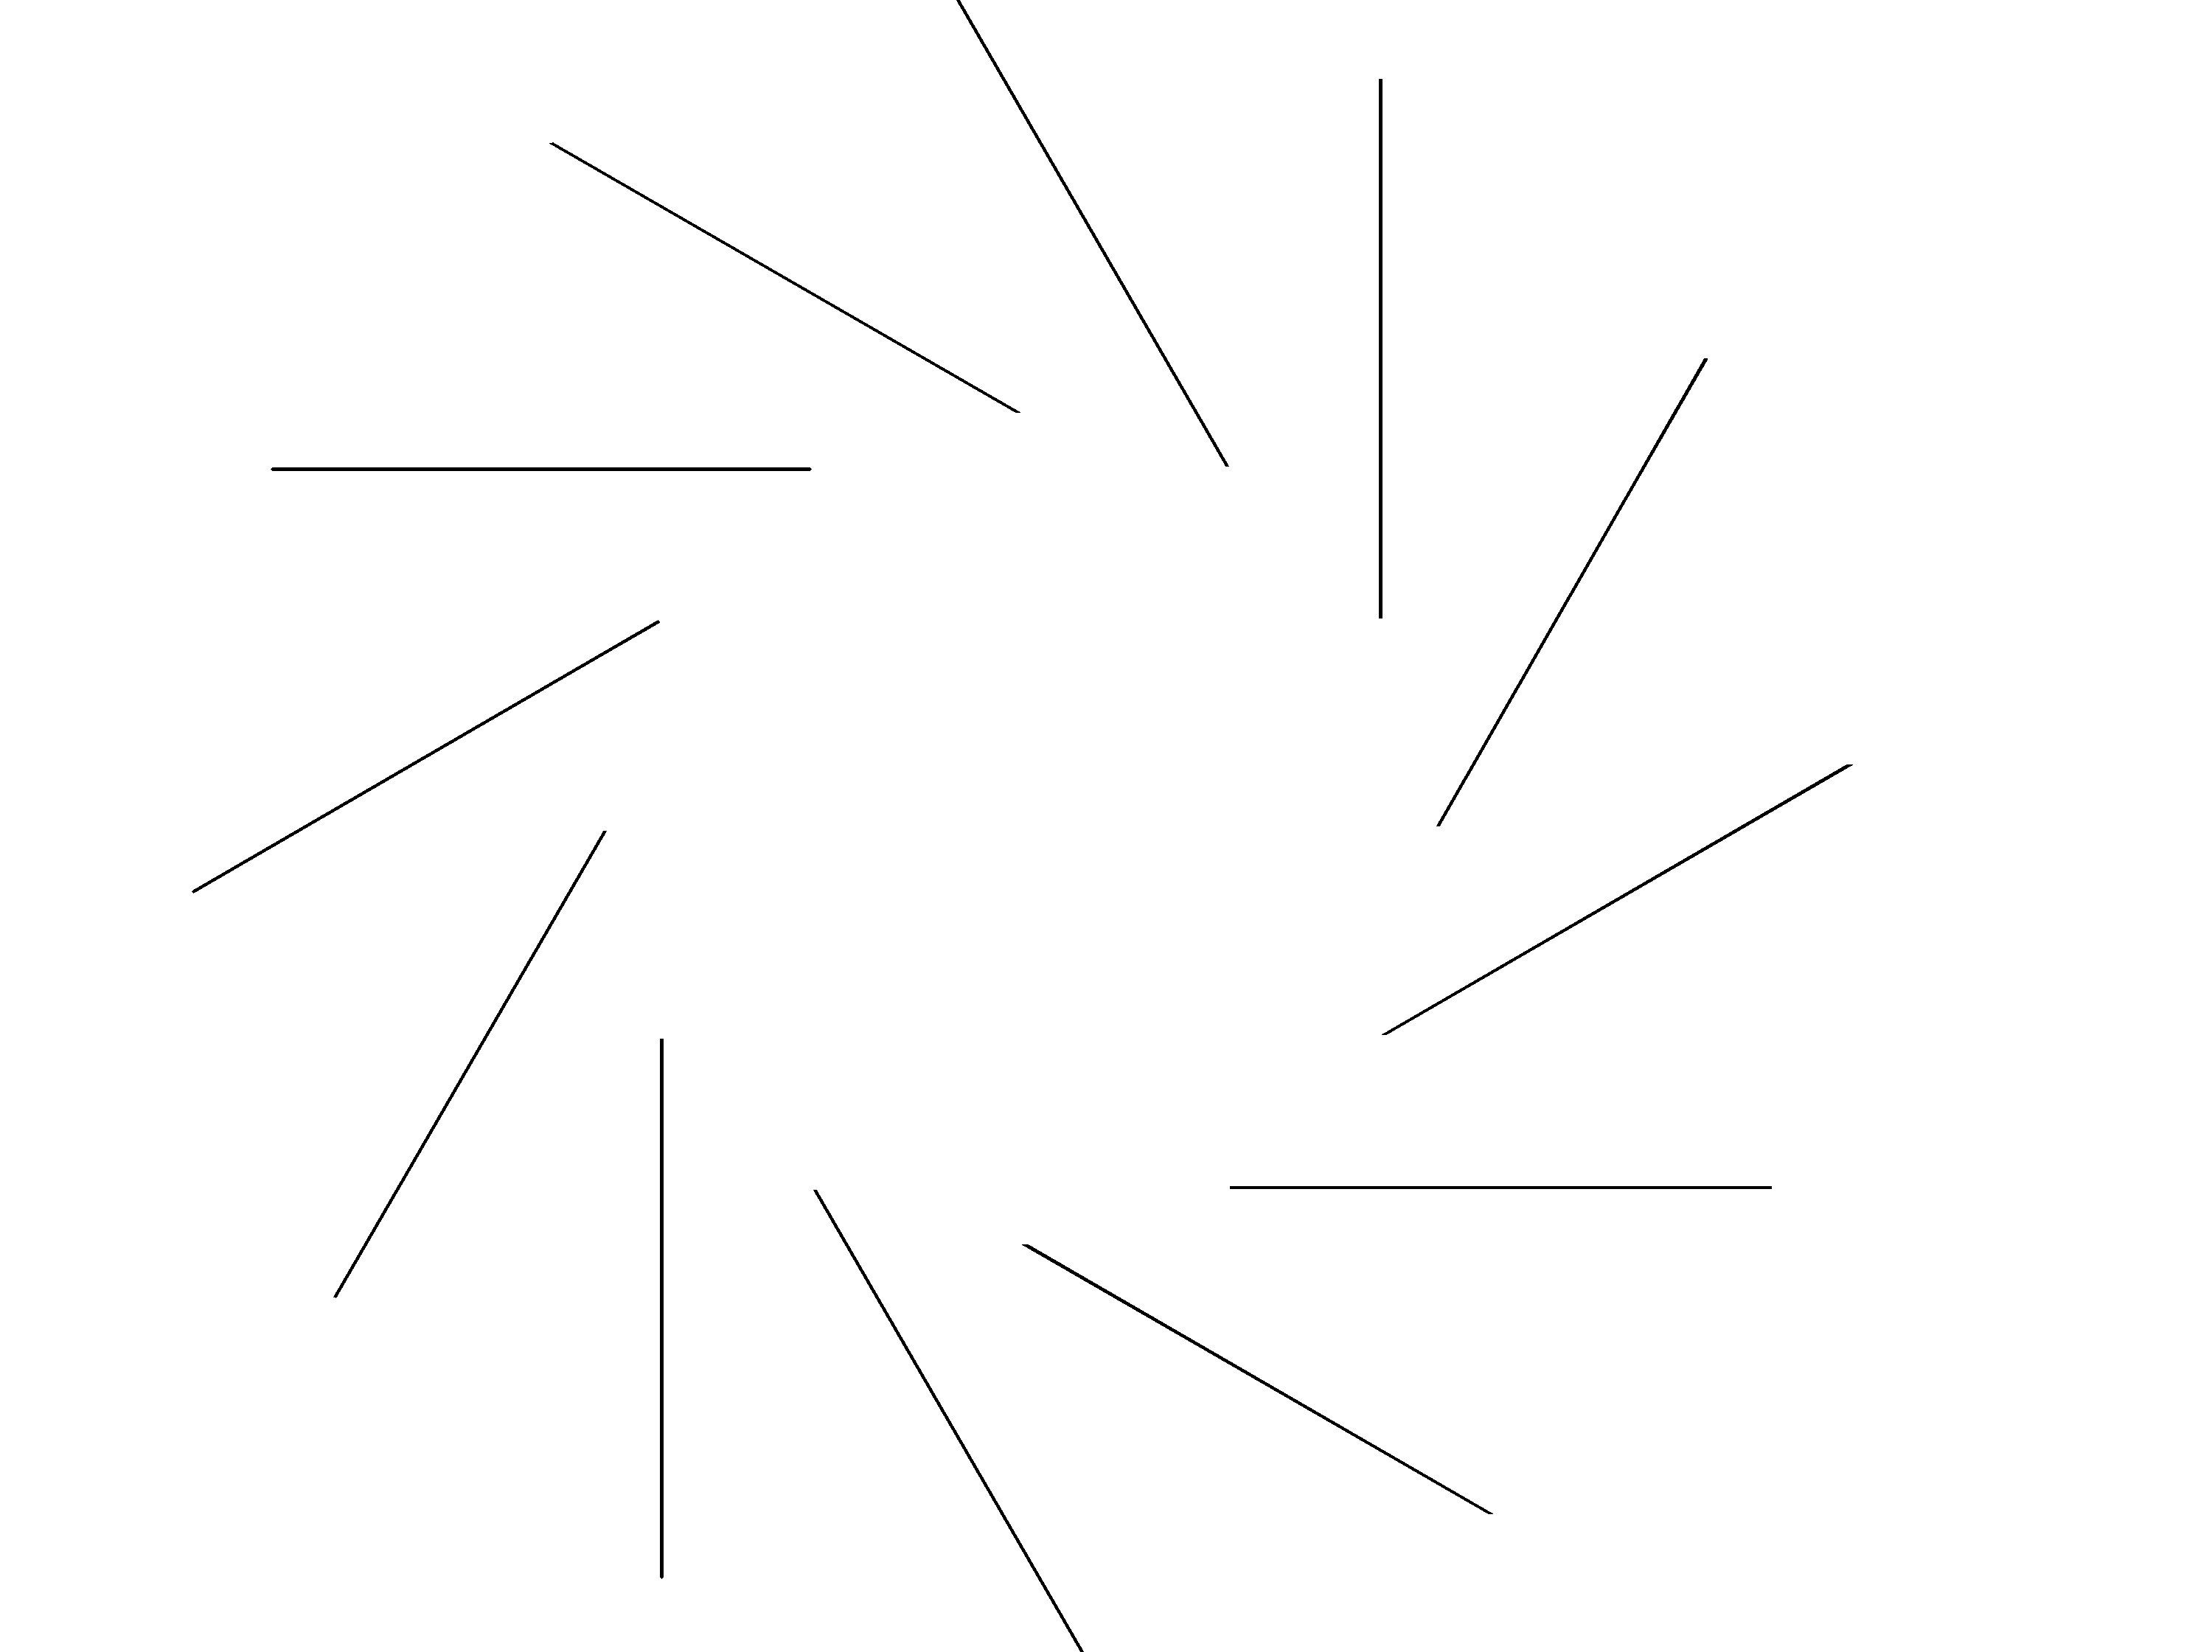
\includegraphics[width =0.47\textwidth]{figs/gridded_region}
    \hfill
    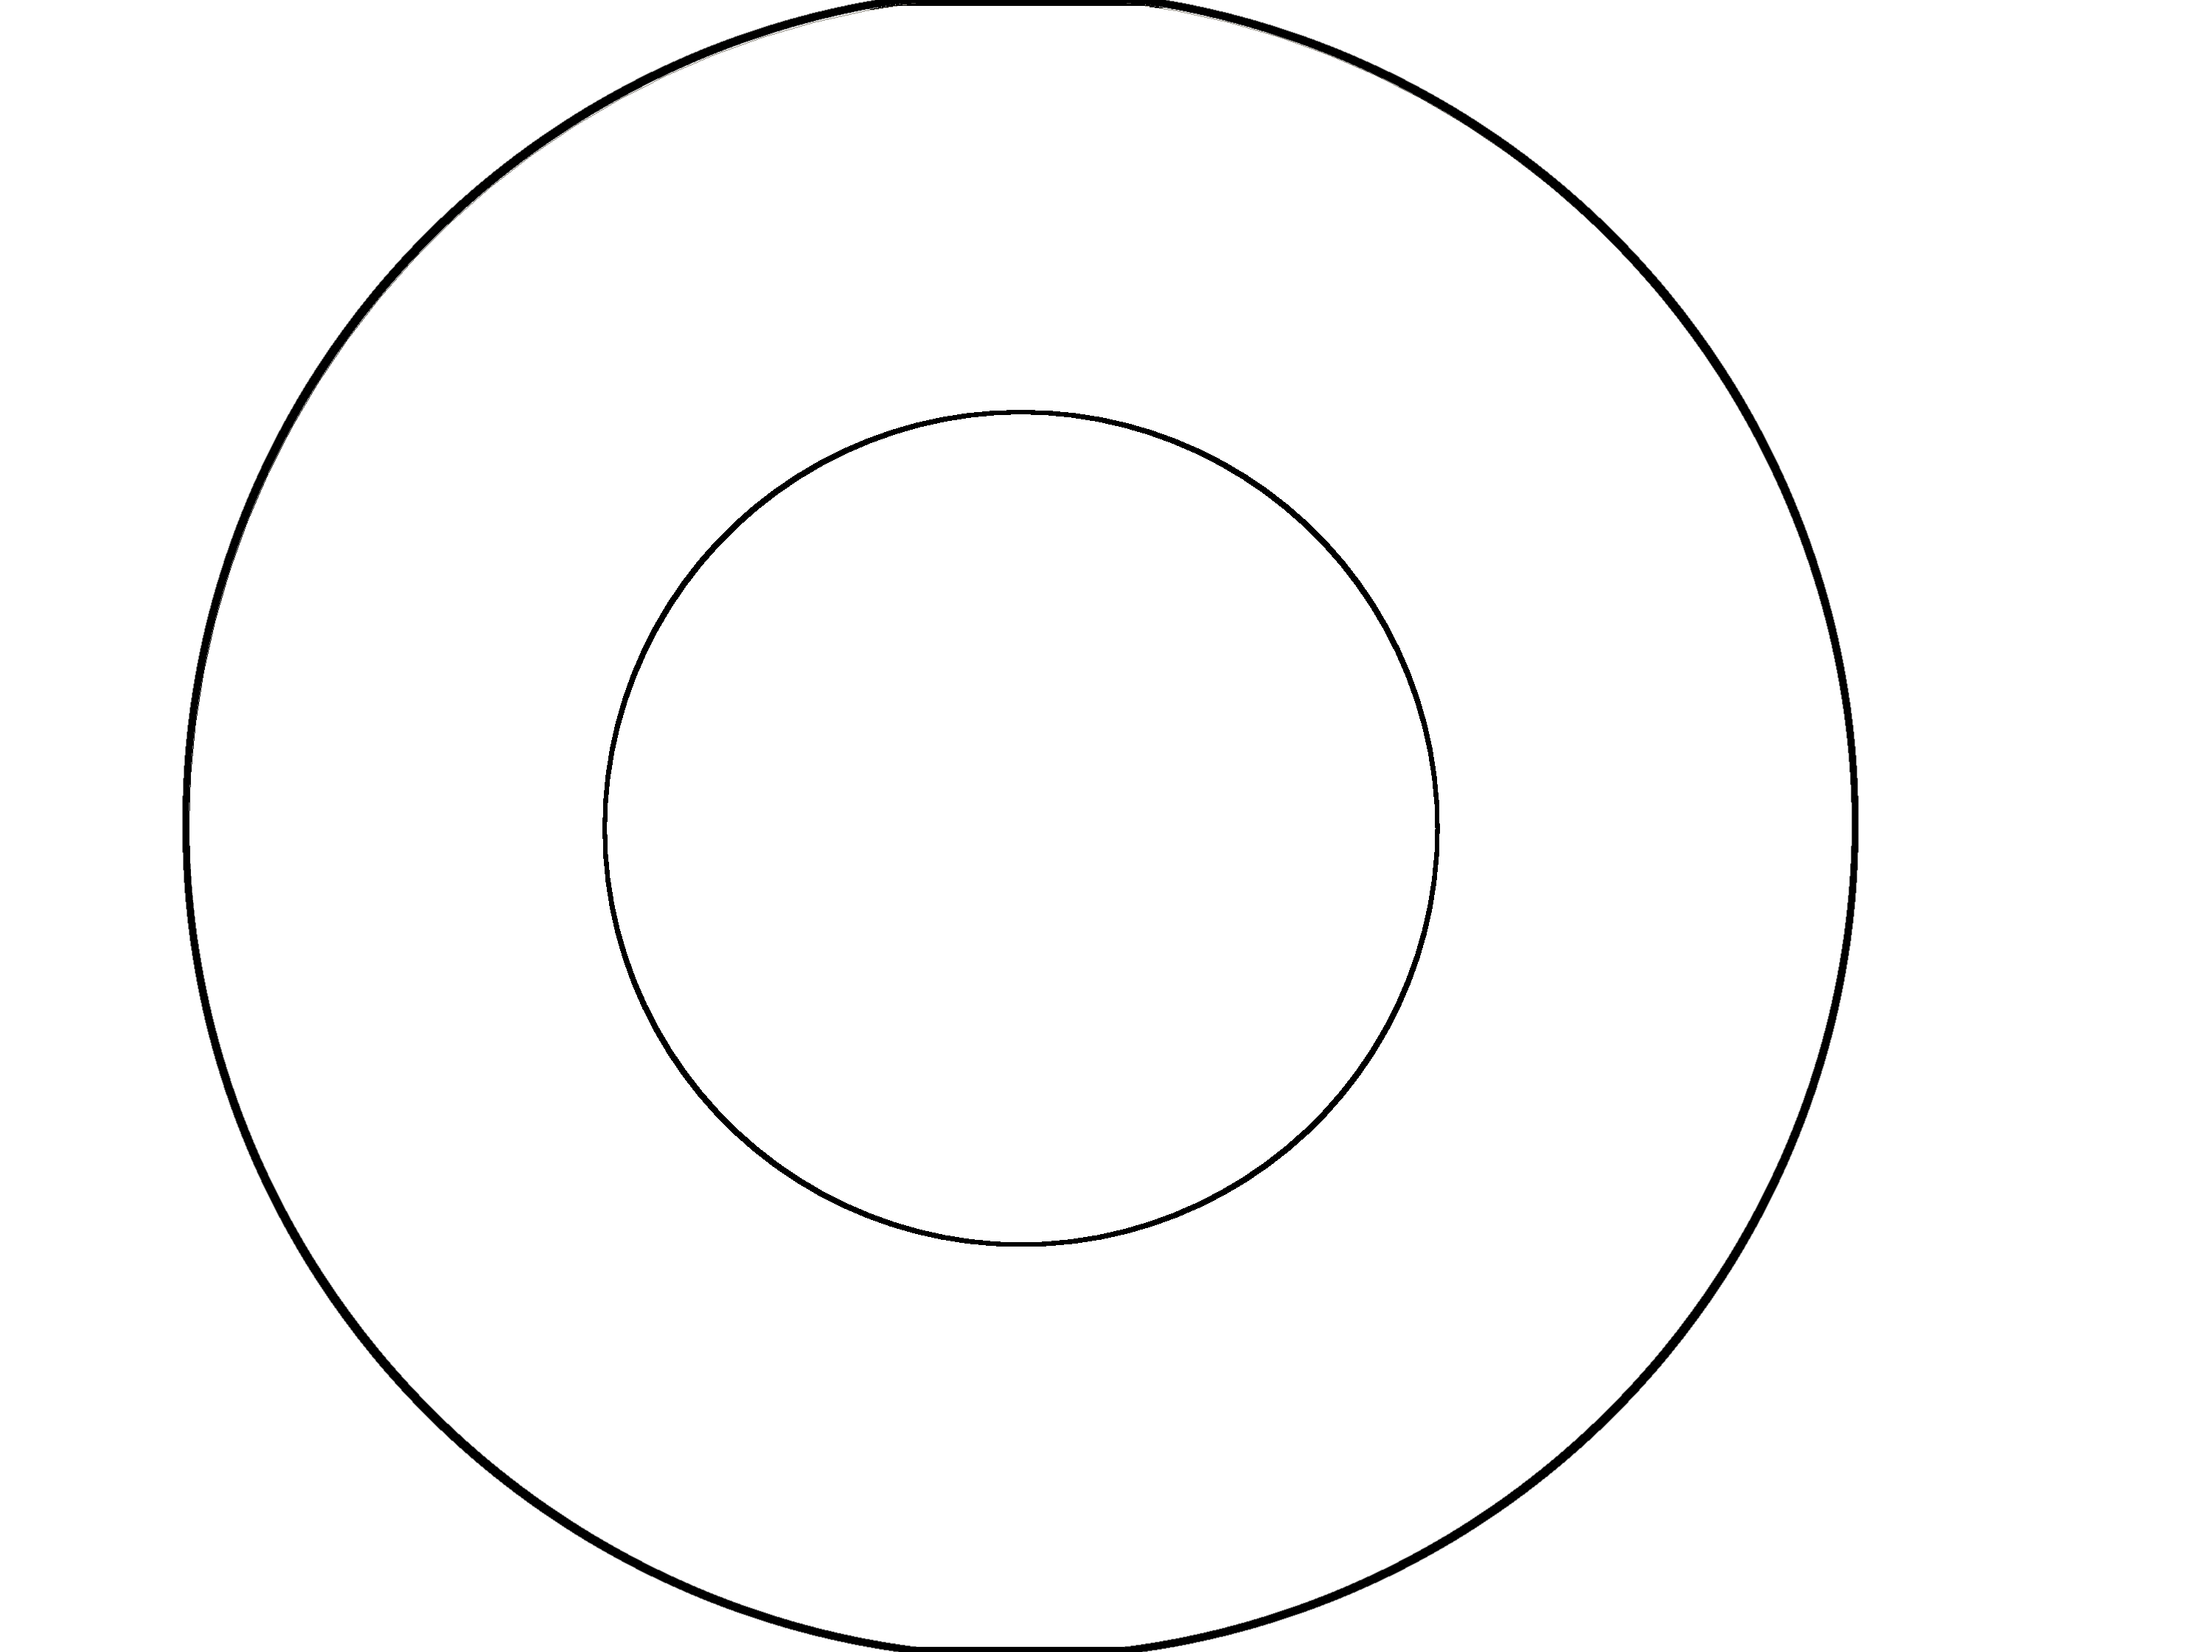
\includegraphics[width =0.35\textwidth]{figs/forcing_region}
     \caption{An example of explicitly represented turning vanes (left)
    versus an annular forcing region (right). $R_{M}$ is the furthest
    radial extent of the virtual vane forcing, and $R_{m}$ the smallest
    radial extent. } 
     \label{fig:penalty_model}
   \end{figure}
%
Vane geometry is specified by the angle $\phi$ a vane makes with a
radial line as a function of the radial coordinate, $r$, and the polar
angle, $\theta$. A unit normal to the vane surface ${\bf n_v}$ is defined
as,
%
\begin{equation}
 {\bf n_v}({\bf x}) = \sin \left(\phi(r,\theta) \right) \hat{{\bf r}}+ \cos
  \left(\phi(r,\theta) \right) \hat{{\bf \theta}},
\end{equation}
%
where $\hat{{\bf r}}$ and $\hat{{\bf \theta}}$ are unit
vectors in the radial and azimuthal directions, respectively.

With this vane-normal vector field specified, a body force ${\bf f_v}$
is defined that will drive the velocity in the ${\bf n}$ direction
toward zero, effectively turning the flow to be parallel to the
vanes. The body force is defined by,
\begin{equation}
 {\bf f}_v= -\frac{1}{\ell_v}|{\bf u}|({\bf u}\cdot{\bf n_v}){\bf n_v},
 \label{eqn:body_force}
\end{equation}
with ${\bf u}$ the velocity and $\ell_v$ is a specified length
scale. The quadratic functional form of this forcing can be motivated by 
the desire for a dimensionally consistent forcing, which is not possible
with only a linear dependence on velocity. The length scale, $\ell_v$,
represents the distance over which the 
flow evolves under the influence of the body force before the
velocity in the normal direction is reduced by a factor of $1/{\bf 
e}$. That is, this is the length over which the normal component of the
velocity decays exponentially. 
%It is the distance analog to the more
%familiar time constant of exponential decay. 

The length scale, $\ell_v$, is a modeling constant and must be
specified. This length scale is calibrated to match the annealing
distance measured in simulations with explicitly meshed vanes. The
length over which the flow comes into alignment with the vane direction
for a gridded vane simulation is measured in
Figure~\ref{fig:annealing}. This plots the average misfit between the
turning vane angle and the fluid velocity, measured as the normalized
difference between the fluid velocity and the tangent line of the
turning vanes. A value of one would represent flow that is perpendicular
to the turning vanes, while a value of zero would represent perfectly
aligned flow.   

The trend is clear that as the flow moves through the turning vanes
towards the center of the apparatus it is brought into alignment with
the turning vane direction. Notice that the misfit actually reaches a
minimum and never comes into complete alignment with the vanes, likely
due to unmodeled transient effects such as vortex shedding off the vane
trailing edges.  

%Our expectation is that it will be the same order as the separation distance
%between neighboring vanes in the physical vane configuration, since
%entry lengths in internal flows scale with the width of the
%channel. 

   \begin{figure}[!htb]
    \centering
    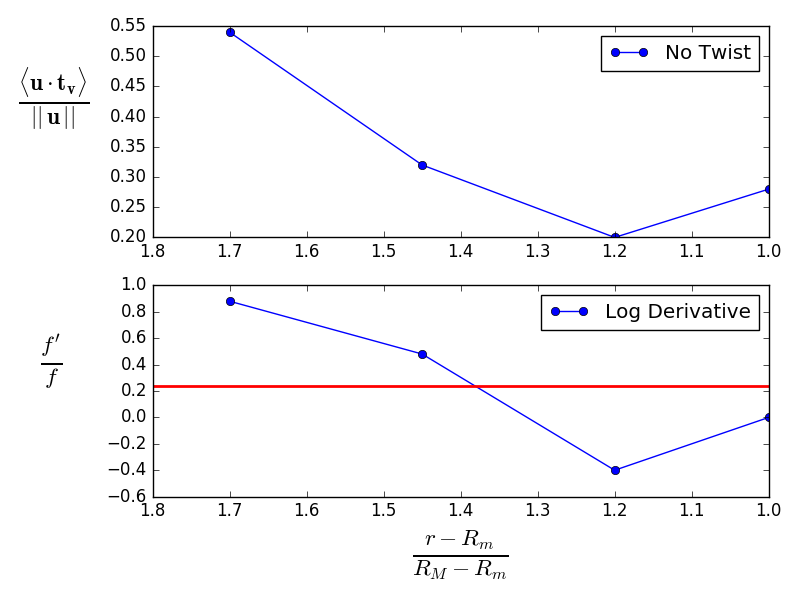
\includegraphics[width =0.8\textwidth]{figs/annealing}
     \caption{The average misfit between the gridded vanes and the
    flow. The averaging is accomplished through azimuthal
    averaging. This was taken at half the height of the turning vanes,
    although the results do not differ at greater or lower height. 
    The subfigure shows the logarithmic derivative in black and the
    average of the logarithmic derivative in red. 
    $R_{M}$ is the furthest radial extent of the gridded vanes,
    and $R_{m}$ the smallest radial extent. The subfigure shows the
    logarithmic derivative of this quantity in black, and the average
    value of the logarithmic derivative in red.}
     \label{fig:annealing}
   \end{figure}

The value of $\ell_v$ is calibrated to explicitly match the 
results of the gridded vanes by assuming that the vane mismatch 
obeys a radial exponential decay of the form $f(r) = A e^{-\lambda r}$, 
where $\lambda = \frac{1}{\ell_v}$.
Taking the logarithmic derivative of this quantity, 
\begin{eqnarray}
 \frac{f'}{f} = \frac{A e^{-\lambda r} * -\lambda}{A e^{-\lambda r}} =
  -\lambda. 
\end{eqnarray}

The logarithmic derivative is shown in the 
subfigure of Figure~\ref{fig:annealing}. If the misfit between vanes 
was perfectly described by an exponential decay, the line would be flat. 
While the curve does not perfectly coincide with this, the curve does
not have severe convexity and the average is sufficient for this
work. Based on this, the lengthscale $\ell_v$ was set to one third of a
meter. 

%\todo{show
%calibration of this} 

This virtual vane formulation is similar to the ``actuator disk'' model
commonly used to represent the rotor of a wind turbine and
described in the subsequent section. 

\section{Turbine Representation}
\label{sec:actuator_disk}
%
% https://en.wikipedia.org/wiki/Blade_solidity
%

The turbine is modeled similarly to the virtual vanes. As with the
vanes, it is desirable to avoid explicitly representing the turbine
blade control surfaces. Instead, the turbine is modeled using the
actuator disc simplification. 
This model (also often referred to as a ``Blade Element Momentum''
theory) is commonly used in wind
turbine design\cite{shevell1983fundamentals,betz,leclerc}. The essence
of this model is to approximate the individual spinning turbine blades
as a ``disk'' in which the effects of the turbine are represented by
body forces on the fluid, as shown in Figure~\ref{fig:actuator_disk}.
This method assumes an axisymmetric representation of the turbine
geometry, and in doing so completely neglects unsteady effects due to
the rotation of turbine blades in a plane. 

As the flow moves through the actuator disk, it experiences a force
normal to the represented turbine blade surface. This force will
generally be in opposition to the flow direction, and will therefore
impart a loss of momentum on the fluid. 
Associated with the loss of axial and azimuthal momentum is a loss of
energy which can be collected by an electrical generator attached
to the rotor shaft if the rotor experiences a torque
in the direction of rotation. 

All the turbine cases shown in this study make the further
simplification that the rotation speed of the disk is constant. 
In this way it is assumed that the turbine exerts a torque equal and
opposite to that of the airflow which keeps the rotational speed
constant. The work done by the aerodynamic torque on the
turbine is assumed to feed into a generator, where it is converted into
electrical energy. 


   \begin{figure}[!htb]
    \centering
    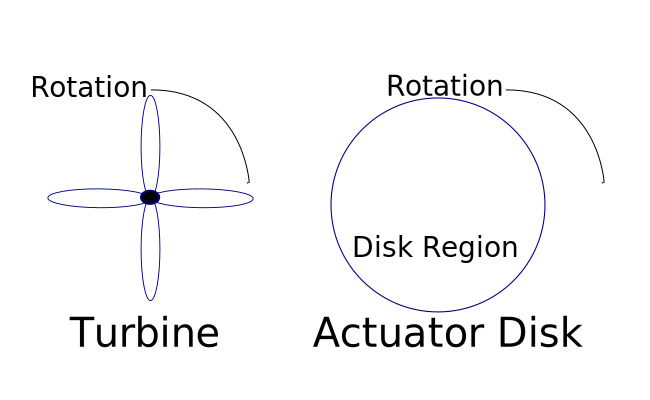
\includegraphics[width =0.95\textwidth]{figs/actuator_disk}
     \caption{The actuator disk model represents a turbine blade
    geometry (shown on the left) as a spinning ``disk'' region (shown
    on the right).}
     \label{fig:actuator_disk}
   \end{figure}

We now detail the mathematical machinery necessary to specify the
direction and magnitude of force between the turbine and flow. The
normal in the blade's velocity direction is, 
\begin{equation*}
n_B = \frac{{\bf u_B}}{||{\bf u_B}||}. 
\end{equation*}
Where ${\bf u_B}$ is the blade velocity vector and is specified. The
normal in the fan vertical direction is typically ${\bf n_f} =
\left(0,0,1\right)$, e.g. pointing ``up''. Then the normal in the radial
direction must be,  
\begin{equation*}
{\bf n_r} = {\bf n_B} \times {\bf n_f}
\end{equation*}

% The fan-wing-plane bit means that we're only looking at the projection
% of velocity into the plane that's defined by the base velocity and
% vertical direction. 

% (01:03:44 PM) Roy Stogner: The "local relative velocity" means that
% we're taking the velocity not in the reference frame of the domain, but
% in the reference frame of the wing.  So if the base velocity is U_B and
% the air velocity is U, then the local relative velocity is U - U_B. 
% (01:04:25 PM) Roy Stogner: Note that we simplify that equation a tiny
% bit by using the fact that U_B and N_R are perpendicular. 

and the fan-wing-plane component (e.g. the plane perpendicular to the 
radius) of local relative velocity is
\begin{equation}
%{\bf u_p} = {\bf u} - ({\bf u}\cdot {\bf n_r})\cdot {\bf n_r} - {\bf u_B}. 
{\bf u_p} = {\bf u} - ({\bf u}\cdot {\bf n_r}) \, {\bf n_r} - {\bf u_B}. 
\end{equation}
This is the projection of velocity into the plane defined by the base
velocity and vertical direction. Now the ``forward velocity'' in the
reference frame of the turbine is,  
\begin{equation}
u_{\text{fwd}} = -{\bf u_p} \cdot {\bf n_B}
\end{equation}
and the ``upward'' velocity in this frame is, 
\begin{equation}
u_{\text{up}} = {\bf u_p} \cdot {\bf n_f}. 
\end{equation}
The angle with respect to the fan velocity direction is then, 
\begin{equation}
% \theta_f = \text{atan2}\left(\frac{{\bf u_{\text{up}}}}{{\bf
 % u_{\text{fwd}}}}\right),
 \theta_f = \text{atan2}\left(\frac{ u_{\text{up} }}{
			 u_{\text{fwd}}}\right), 
 %\theta_f =
  %\text{tan}^{-1}\left(\frac{u_{\text{up}}}{u_{\text{fwd}}}\right)
  \label{eq:fan_direction}
\end{equation}
while the angle with respect to the chord is this with the addition of
the blade angle relative to the fan vertical direction, 
\begin{equation}
 \phi = \theta_f + \beta(r).
\end{equation}

In words, the blade angle (or local pitch) is measured from the plane of
rotation to the chord line (i.e., the straight line connecting leading
to trailing edge). These parameters, $\beta$, C, etc. are visually
depicted in Figure \ref{fig:turbine_image}.  

The actuator disk model assumes that the forces on a blade
element can be calculated by means of two-dimensional aerofoil
characteristics using an angle of attack determined from the incident
resultant velocity in the cross-sectional plane of the element. The
velocity component in the span-wise direction is
ignored. Three-dimensional effects are also
ignored\cite{burton2001wind}.  

  \begin{figure}[!htb]
    \begin{center}
     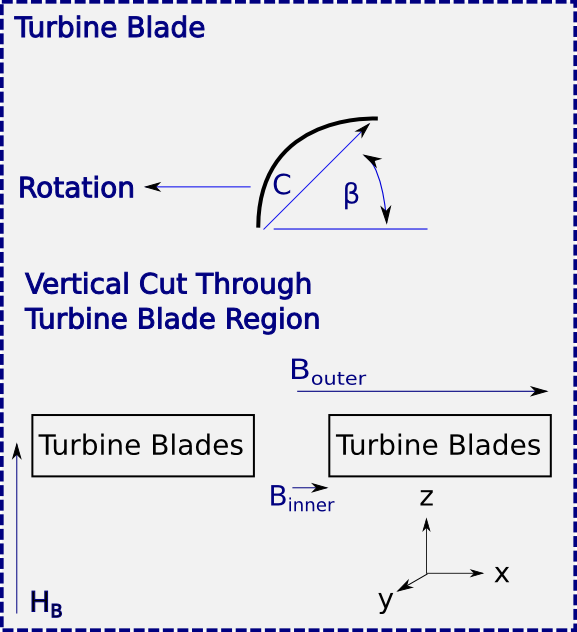
\includegraphics[width = 10 cm]{figs/turbine_image}
     \caption{The represented turbine blade
     geometry. $\beta$, the blade angle, is measured relative to the
     horizontal plane. c, the chord length of the turbine, is defined as
     the straight line distance from leading to trailing edge. } 
     \label{fig:turbine_image}
    \end{center}
  \end{figure}

\subsection{Specification of the Lift and Drag Coefficients}

We now define the lift and drag normals, where the direction opposing
drag is, by definition,  
\begin{equation}
{\bf n_{\text{drag}}} = \frac{{\bf u_p}}{||{\bf u_p}||} 
\end{equation}
and the direction opposing lift orthogonal to the drag and the radial 
direction,  
\begin{equation}
{\bf n_{\text{lift}}}= {\bf n_{\text{drag}}} \times {\bf n_r}. 
\end{equation}
%
Then, the force on the turbine is, 
% \begin{equation}
%  \boxed{F = \frac{1}{2}\frac{\rho u_p^2 c}{A}\left(C_l \cdot
% 					      n_\text{lift} + C_d \cdot
% 					      n_\text{drag}  \right)}
% \label{eq:force_turb}
  % \end{equation}
\begin{equation}
 F = \frac{1}{2} \rho A_B {\bf u_p}^2 \left(C_l \,
					      {\bf n_\text{lift}} + C_d \,
					      {\bf n_\text{drag}}  \right).
\label{eq:force_turb}
\end{equation}
$A_B$ is the total area of the turbine blades, so $A_B = B\, c\, r$, where B
is the number of turbine blades and c is the chord length of the
turbine. 
The actuator disk is an approximation of the blades as a volumetric
forcing ``disk'', and so our interest is in this quantity,
\begin{equation}
\frac{F}{\text{volume}} = \frac{F}{\pi r^2 t} = \frac{1}{2}\frac{\rho\, B\, c\,
 {\bf u_p}^2}{\pi r t}\left(C_l \, {\bf n_\text{lift}} + C_d \, {\bf
		   n_\text{drag}} \right).  
\label{eq:vol_turb}
\end{equation}
Where t is the blade thickness of the actuator disk.
Note that the volume is over a different extent than the area. The
volume is for the entire actuator disk, while the force on the blades
was only calculated with total surface area of the turbine. 
To better understand this, note that the product $B c$ appears in
Equation~\ref{eq:vol_turb}, above. This quantity impacts the solidity (or
blockage), and as the chord length or number of blades increases,
the total blocked area inside the actuator disk also increases. It is
interesting to note that in the actuator disk model, only the product $B c$
has impact, and one cannot directly separate the impact of more turbine
blades versus larger blade chord lengths. 
The impact of solidity will be discussed in greater detail in
Section~\ref{sec:solidity}.

Now, only the drag coefficients ($C_l,C_d$) must be specified to fully
determine the force on the blades. These coefficients are functions of
the angle of attack, $\alpha$. Data for the coefficients was provided
by Duane McCormick at UTRC and were generated from a 2-D model in
COMSOL. As the data was discrete, high order polynomials were used
to obtain smooth functions fit to the COMSOL data. Typically,
16\textsuperscript{th} order polynomials were used to 
ensure that the fitted function closely matched the provided
data. The drag and lift functions for the three cases considered (flat
plates, $180^{\circ}$, $90^{\circ}$ circles) are shown in 
Figures~\ref{fig:flat_plate_drag}, \ref{fig:semi_drag} and
\ref{fig:90_drag}. The flat plate drag coefficient is smoothly
varying and so the interpolated function is close to the provided
data. The semi-circles ($180^{\circ}$) are largely accurate, but near
zero degrees the COMSOL data for the lift function shows a sharp feature
that is not well resolved by the interpolating polynomial. This is also
the case for the quarter-circles, where near a zero angle of attack the
lift function has a near discontinuity that is not well resolved by the
interpolated function. 

%The semi-circular plots are more complicated. Here, we use a high order
%polynomial fit to continuously interpolate between drag polars. 

\begin{figure}[!htb]
  \begin{center}
    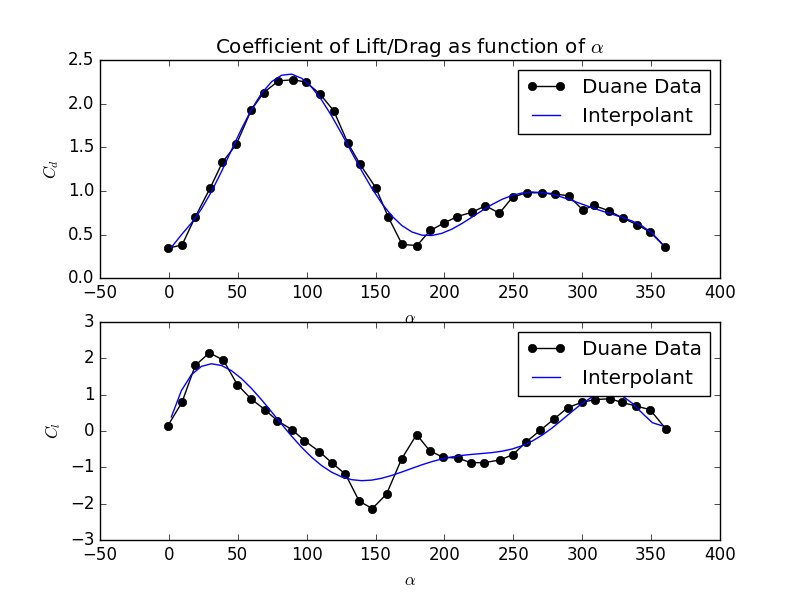
\includegraphics[width = 12 cm]{figs/flat}
    \caption{The flat plate lift and drag coefficients as a function of the angle of attack, $\alpha$.} 
    \label{fig:flat_plate_drag}
  \end{center}
\end{figure}

\begin{figure}[!htb]
  \begin{center}
    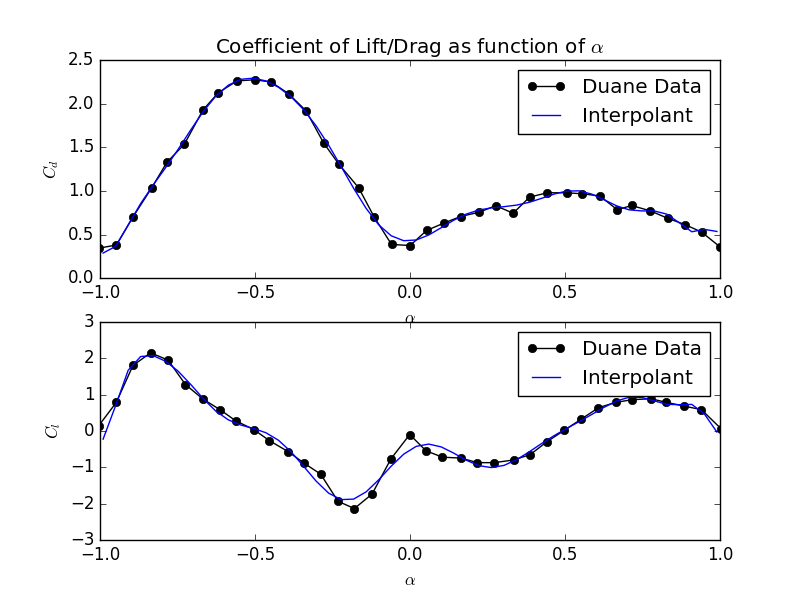
\includegraphics[width = 12 cm]{figs/semi}
    \caption{The semicircle (180 degree) lift and drag coefficients as a function of the angle of attack, $\alpha$.} 
    \label{fig:semi_drag}
  \end{center}
\end{figure}

\begin{figure}[!htb]
  \begin{center}
    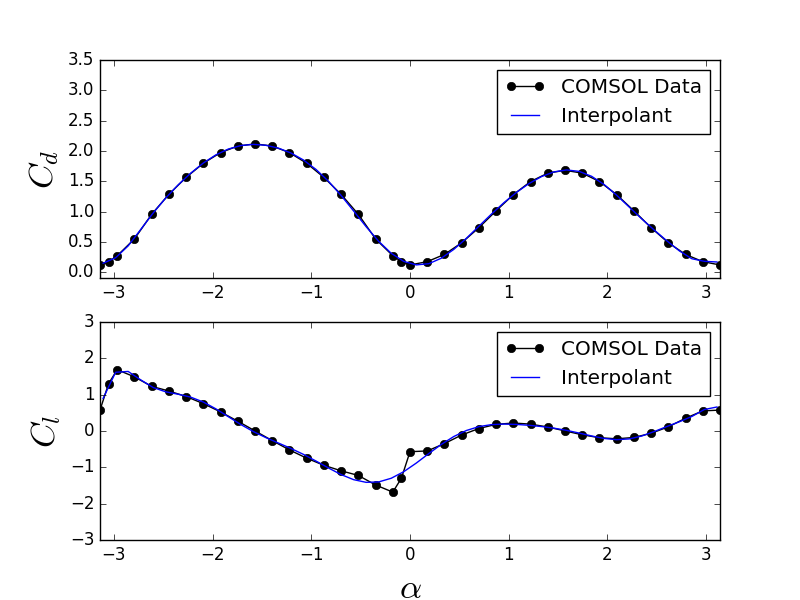
\includegraphics[width = 12 cm]{figs/90}
    \caption{The 90 degree (quarter circle) lift and drag coefficient as a function of the angle of attack, $\alpha$.} 
    \label{fig:90_drag}
  \end{center}
\end{figure}

% what about loads on turbine?\todo{loads?}
% Blade torque loads modest, only ~20 ft-lbs
%% load was predicted at 20 ft*lbs

% lets kill this one
%\subsection{Shortcomings of the Actuator Disk Model}
%\label{subsec:wake_loss_model}

The actuator disk model is valuable because of its simplicity, not on
account of its accuracy. Despite its pervasive use, there are numerous
known inadequacies to the model. 

% In particular, the actuator disk does not account for the separation of
% flow between blades, and implicitly assumes the flow remains attached. 
% This model deficiency results due to the actuator disk
% method's dependence on the precision of the lift and drag
% coefficients. During the operation of a wind turbine, should the angle
% of attack reach high values (post-stall region), then aerodynamic
% data is not available or inaccurate.  
% This model inadequacy is commonly fixed with the Glauert Correction. 
% Developed in 1926 by Glauert from helicopters rotor blades, this
% correction originally was purely based on experimental data. The model
% was designed to correct the overall thrust coefficient for high angles
% of attack\cite{glauert1926general,glauert1935airplane}. 
% While the Glauert correction is a tip loss model, the correction was
% developed as a correction to an entire rotor disk; the original
% researcher did not intend it to be applied to a rotor annulus. 
%Given that 
%a duct eliminates tip losses\todo{write me}
%However, because of a limited amount of experimental data, an alternative model does not exist.  

For instance, the model's described above account for the turbulent wake
state, which in some cases have been shown to be significant for a wind
turbine\cite{churchfield2012numerical} and may have substantial impact
on the SoV. 

Various researchers\cite{Moriarty_aerodyntheory,wilson1978design} have
suggested various other corrections to actuator-disk theory. These
corrections include (among others) accounting for blade thickness on
local angle of attack, cascade width for high solidity turbines, and
spanwise gaps for partial span pitch control. The impact of these
missing physics can be significant, for instance, blade thickness
can be aerodynamically significant near the rotor hub and may 
affect the in-plane forces on the rotor. Nevertheless,
these corrections are not treated in the simulations presented in this
document. 

In summary, the actuator disk is a useful modeling tool for this study
but does not represent a high-fidelity representation of the turbine
blade dynamics, and should not be considered highly accurate. Attempts
to evaluate and characterize these shortcomings are detailed in
Chapter~\ref{sec:field}.  Additionally, a new modification to the
actuator disk that modifies the model to further account for blade
solidity is demonstrated in this work in Section~\ref{sec:solidity}. 

\section{Solid Surface Representation}
\label{subsec:solid_surface}

In addition to vanes, the SoV device includes impermeable surfaces
such as the wind break (``cone'') on the top of the facility. As with
the turning vanes, this is represented without explicitly meshing the
surface nor imposing  a boundary condition at the surface. This allows
rapid exploration of configurations  with different solid surfaces to
control and manipulate the fluid flow. These solid surfaces are
represented by a body force acting in a region surrounding the wall. 
A body force normal to the surface is defined in this region so
that it will drive the normal velocity to zero, resulting in the flow
moving only parallel to the virtual surface. 
The body force is defined as in Equation
\ref{eqn:body_force}; however, the length scale $\ell_v$ is specified to
be the width of the forcing region used to represent the surface. This is
typically the width of two or three grid cells. While the actual surface we are
emulating is thinner than this, the numerical discretization 
cannot represent anything thinner. 
%difficulty converging for surfaces smaller than the grid size.  

Forcing models designed to mimic a surface are not original to this
 project, and the current formulation is  closely related to (among others)
``immersed boundary methods'' as used by various other
researchers~\cite{doi:10.1146/annurev.fluid.37.061903.175743,verzicco1998complex}. This
approach is unique in its use of Babuska's penalty treatment of
constraints\cite{1973fempen,ZAMM:ZAMM19880680925} to enforce the
behavior at the boundary. This method was selected because it is easily
imposed in the FEM context, and the penalty method properties have been
explored in detail in the literature.
%\todo{add more discussion of
%healing length implications here} 
Note that despite the similarity in name, this is a distinct technique
from the ``penalty immersed boundary method'' of Kim and
Peskin\cite{:/content/aip/journal/pof2/19/5/10.1063/1.2734674}.  

%show image of cylinder in 2d flow?\todo{add cylinder image? what does
%zthis show?} 

%Typically, the enforcement occurs along a domain
%boundary, but in this work it is used in the interior, 
%and is not imposed as a mathematical constraint but rather as a modeling 
%approach. 

% We add a penalty term to the weak
% form of the Navier-Stokes momentum equation described in the subsequent
% section %\ref{eq:ns_weak} 
% that has the form, 
% \begin{equation}
% P_\epsilon = \int_\Omega ({\bf f_v} \cdot v) \, dx
% \end{equation}
% where ${\bf f_v}$ is as described in equation \ref{eqn:body_force}. 
%% As the system is formulated as a variational problem that seeks to
%% minimize the test function $v$, any velocity that is not aligned with
%% the vane normal will incur a penalty versus one that does. Note that unlike
%% some penalty methods, this does not automatically satisfy
%% continuity. Rather, the velocity field remains divergence free through a
%% separately enforced constraint.  

\section{Separation Model}
\label{sec:separation}

In the presence of wind, it was found that there was a significant flow
out through the vanes in the back of the device. This was obviously
inconsistent with the findings of our colleagues in the field, who
observed no such outflows. Moreover, this resulted
in large inconsistencies between our predictions and the field results,
almost certainly because of the kinetic and thermal energy that our vane
representation was permitting to leave out the back of the device.  

This exposed a weakness of the turning vane representation outlined
previously. When the flow entered the virtual vane forcing region it was
always turned to align with the vane angle, even when the forcing was in
the opposite direction of the present velocity.
This is in contrast to the physical situation, in which we
expect the flow to continue along an averaged streamline separating from the 
trailing edges of the vanes, instead of turning around it. 
The averaged streamline will continue past the trailing edge of the vane
due to the separation of the boundary layer off the edge surface. An
image depicting these two cases in shown in Figure \ref{fig:sep_model}.  

\begin{figure}[!htb]
  \begin{center}
    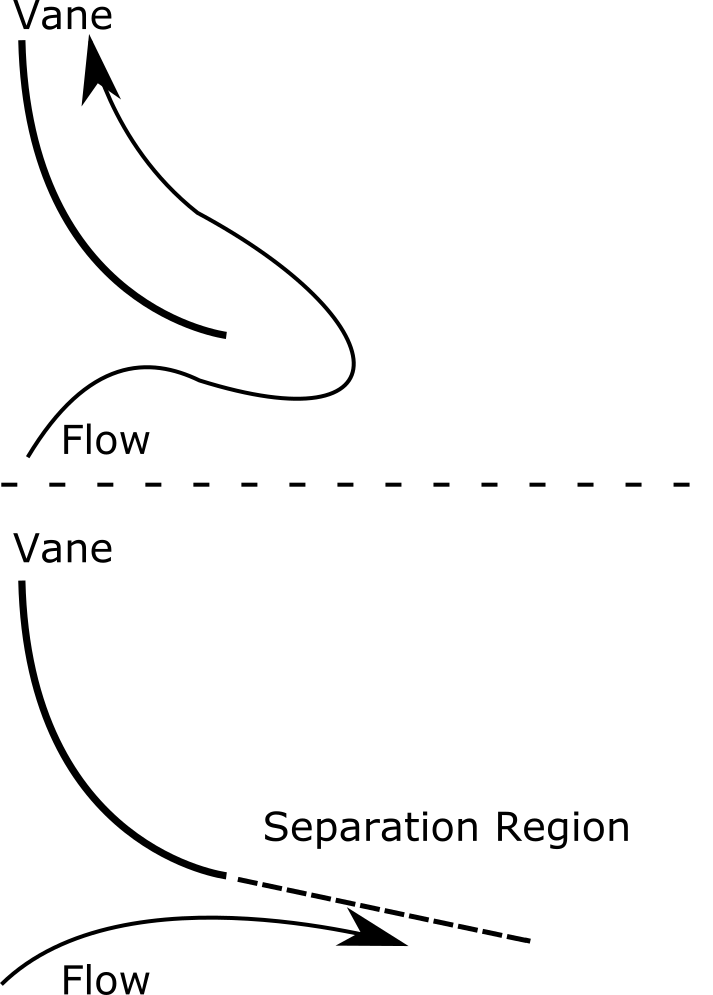
\includegraphics[width = 6 cm]{figs/sep_model}
    \caption{Schematic depicting the separation model that extends past
   the trailing edge of the vanes. In the top case, the flow entering
   the virtual vane region is forced to align with the vane angle despite
   this resulting in a reversal of the flow direction. This is a
   consequence of the forcing function acting on the fluid to ensure the
   velocity vector aligns with the vane. 
   The second case depicts the separation
   model, where the flow under certain conditions is not forced and
   continues to move tangent to the vanes due to 
   the separation of the boundary layer off the trailing edge.} 
    \label{fig:sep_model}
  \end{center}
\end{figure}

Let $\bf n_v$ be the normal vector to the vanes,
and $\bf n_r$ the normal vector pointing out of the vane
region\footnote{\normalsize The subscripts ``v'' and ``r'' stand for
vane and radial, respectively.}.  
Then, $\bf t_v$ is the tangent vector to the vanes pointing out of
the vane region and is defined as,

%\begin{equation}
% \bf t^v = \left( {\bf n^v_y},{\bf -n_x^v} \right) \text{sign}\left[
%	    \left( {\bf n^v_y},{\bf -n_x^v} \right) \cdot {\bf n^r} \right].
%\end{equation}
\begin{equation}
 \bf t_v = \left( {\bf n_v^{\perp}} \right) \text{sign}\left(
	    {\bf n_v^{\perp}} \cdot {\bf n_r} \right).
\end{equation}
Here, sign() is the sign (or signum) function, that extracts the 
sign of a real number and ${\bf n_v^{\perp}}$ is the vector 
perpendicular to the normal vector of the vanes, which is simply, 
\begin{equation*}
 {\bf n_v^{\perp}} = \left[ \begin{array}{c}
n_x\\
n_y\\
\end{array}\right]^{\perp} = 
 \left[ \begin{array}{c}
  -n_y\\
  n_x\\
	\end{array}\right].
\end{equation*}

%
% example of an algorithm
%

% \begin{center}
%  \begin{algorithm}
%   \caption{The crude separation model. This model identifies if the flow
%   is coming into or out of the vane region, and if the velocity vector
%   is in the same direction as the tangent line of the vanes. In the case
%   of the ``special forcing'' the flow is forced as if it was
%   impacting a solid surface. In the
%   algorithm below, $r_0$ is the max radius of vanes, $r_i$ the minimum
%   radius of vanes, and $\delta$ is the width of the separation region.}
%   \label{alg:sep}
%   \begin{algorithmic}
%    \IF{($r_0 > r > r_i$)} 
%    \IF{$(r_0 - r) < \delta$ \textbf{or} $((r - r_i) < \delta)$}
%    \STATE ${\bf n_r} = {\bf r}/|r|$
%    \IF{$(r - r_i) < \delta$} 
%    \STATE ${\bf n_r} = -{\bf n_r}$
%    \ENDIF
%    \STATE  $\bf t_v = \left( {\bf n_v^{\perp}} \right) \text{sign}\left(
%   	    {\bf n_v^{\perp}} \cdot {\bf n_r} \right)$
%    \IF{$v \cdot t_v > 0$ \textbf{and} $v \cdot n_r < 0 $}
%    \STATE ${\bf n}({\bf x}) = \hat r$ \quad (Special Forcing)
%    \ELSE
%    \STATE  ${\bf n}({\bf x}) = \sin \left(\phi(r) \right) \hat{{\bf r}}+ \cos
%   \left(\phi(r) \right) \hat{{\bf \theta}} $
%   \quad (Normal Forcing)
%    \ENDIF
%    \ELSE
%    \STATE ${\bf n}({\bf x}) = \sin \left(\phi(r) \right) \hat{{\bf r}}+ \cos
%   \left(\phi(r) \right) \hat{{\bf \theta}} $
%   \quad (Normal Forcing)
%    \ENDIF
%    \ENDIF
%   \end{algorithmic}
%  \end{algorithm}
% \end{center}


The forcing is modified when the velocity vector of the local flow, ${\bf u}$ 
is pointing into the forcing region: ${\bf u} \cdot {\bf n_r} < 0$, and
when the velocity vector is in the same direction as the tangent line to
the vanes: $ {\bf u} \cdot {\bf t_v} > 0 $, 

\begin{equation}
 {\bf n}({\bf x}) = 
 \begin{cases} 
   \hat {\bf r}  & \text{if } {\bf u} \cdot {\bf n_r} < 0 \text{ and }  {\bf u} \cdot {\bf t_v} > 0  ,\\
   \sin \left(\phi \right) \hat{{\bf r}}+ \cos \left(\phi \right) \hat{{\bf \theta}}  & \text{else}.
 \end{cases}
\end{equation}
%
In these instances, the
forcing acts as if there was a rigid surface past the vane edge, and
gives the appearance of a special ``no-penetration'' condition for the
velocity for these cases. 

%The pseudo-code for this procedure is shown in
%Algorithm~\ref{alg:sep}.\todo{cant write mathematically, would be easier}

The addition of this simple separation model significantly reduced the
flow that penetrated the back of the vanes, and produces results
consistent with the observations provided by our experimental
colleagues.  

\section{Effect of Surface Roughness}

%%
%% this does not describe the phenomena being modeled or the precise
%% model -- rewrite
%%
%%
%% this does not say enough about the surface roughness
%% motivate that and explain how it is used, than show your estimate 
%% to argue it is small
%%

Surface roughness effects have been shown to play a role in the
formation of dust devils and related atmospheric
phenomena\cite{oke1987boundary}. For the flat and sandy
regions we are simulating, the impact is expected to be a small vertical 
velocity perturbation which triggers the convective instability caused
by stratification near the surface. 
%a small
%``kick-up'' forcing velocity perturbation in the vertical
%direction. 
Assuming azimuthal symmetry, this is modeled as a volumetric forcing in
a narrow region above the surface in the region of the vanes,  
\begin{equation}
 F^{'''}_{z_0} = \frac{1}{2}\rho V_f^2/z_{0}, 
\end{equation}
where $z_{0}$ is the forcing region height and $V_f$ is the magnitude of
 the  induced velocity fluctuation which is estimated as, 
%\begin{eqnarray}
%z_0 = \frac{1}{2} a t^2, \\
%t = \sqrt{\frac{2 a}{z_0}}. \\
%\end{eqnarray}
%Combining this with, $V_f = a t$, our estimate is, 
\begin{equation}
V_f = \sqrt{2 a z_0}.
\end{equation}
The forcing region height $z_0$ is set to the boundary layer thickness
of 10 centimeters. The acceleration was estimated at 0.05
$\text{m}/\text{s}^2$, based on the observed surface roughness impact on
tornado-like vorticies of Natarajan and Hangan\cite{Natarajan2012577}.

We ensure that the energy
introduced into the flow is a small fraction of total flow energy by comparing
this with the energy flux through the top of the vanes. The total energy
added is measured as,  
\begin{equation}
 E_{\text{injected}} = \int_0^{2\pi} \int_0^R \int_0^{z_0} F^{'''}_{z_0}
  dz dr d\theta.  
\end{equation}
R is the outer diameter of the vanes. 
The value of $E_{\text{injected}}$ is typically a few percent of the
total kinetic energy flux measured through the top of the
vanes.

Leslie~\cite{leslie1977surface} and Dessens~\cite{dessens1972influence}
found that the introduction of surface roughness effects caused a slight
decrease in tangential velocity for simulated vortices, but an increase
in radial and axial velocities. 
On a related note, hurricane studies have
consistently found enhanced heat transport near the surface lead
to storm intensification, indicating an important role due to roughness
effects~\cite{Zeng2010,GRL:GRL50047,hurricane_drag}. The interaction
with the surface and therefore, the impact of roughness, is likely
complicated and is not considered in detail in this work. It should be 
noted that in the simulations performed in the course of this study, the
surface roughness model was observed to modestly intensify the thermal
vortex, typically by several percent. While this formulation was
undoubtedly {\it ad hoc}, studies performed on representative test 
cases found that results were not sensitive to small
changes in the forcing region height, radial distance, or
forcing magnitude. 

%This general forcing provides additional capabilities including the
%ability to investigate engineering greater surface roughness or
%structures that could provide greater ``kick-up'' of the thin thermal
%layer near the surface into the flowing regime. It can also support more
%general turning configurations than the virtual vanes outlined above. 

\section{Simulation Geometry and Boundary Conditions}
\label{sec:bc}

In this project, two principle modeling regimes are considered.  
One is the ``thermal-only'' scenario, in which there is no wind
 and there is an imposed elevated temperature on the ground.  
In the other, there are also ambient winds that contribute to the SoV energy
(``wind'' cases) and elevated ground temperature. 
The computational domain and boundary conditions for these 
two scenarios are described below.

%\subsection{Computational Domain} 
\textbf{Computational Domain} 

All simulations are performed in a cuboid domain, with six
faces.  The domain is denoted $\Omega \subset \mathbb{R}^3$. 
The domain extents are scaled by the system diameter, D, created by the
outer vane radius. The extents are defined in terms of $\{L_x,L_y,L_z\}$ indicating the 
streamwise, spanwise and vertical directions, respectively. 
For both simulation regimes, sensitivity analyses 
were performed to ensure that the results were not sensitive 
to the domain extents. For the thermal-only case, for which $L_x = L_y$,
the system 
extents $L_x/D$ and $L_y/D$ are chosen to be 3. The height ($L_z/D$) is
three times the system diameter, which is typically nearly equal to the
height of the vanes. This defines the thermal-only domain $\Omega_T$, 
as $\Omega_T = \left[-L_x,L_x \right] \times \left[-L_y,L_y \right]
\times \left[0,L_z \right]$.   

For the wind cases, the streamwise extent is no longer equal to
the spanwise length, $L_y$. In these cases, the domain length extends
two diameters in front of the vanes and three behind. The
spanwise direction is symmetric and extends two diameters in each direction 
from the center ($L_y/D = 2$). The height is identical to the
thermal-only case, at three system diameters ($L_z/D = 3$). Thus, the
wind domain is defined as $\Omega_W = \left[-2D,3D \right] \times
\left[-L_y,L_y \right] \times \left[0,L_z \right]$.   

The boundary for the thermal only case is decomposed as,
$\partial \Omega_T = \Gamma_G \, \bigcup \, \Gamma_T \, \bigcup \,
\Gamma_P $.  
$\Gamma_G$ is the boundary along the ``Ground'', $\Gamma_T$
the ``Top'' boundary, and $\Gamma_P$ the four periodic ``Sides''. A 3D
diagram labeling these boundaries appears in
Figure~\ref{fig:thermal3d}. For this case (no mean wind),
periodic boundary conditions are used on the four sides , with a modified 
``inflow-outflow'' Neumann condition\cite{gunzburger1989finite} on the
top boundary. On the ground, a ``no-slip'' velocity boundary condition is
imposed, and a Dirichlet condition uniformly fixes
the temperature of the surface. 
Each of the $\Gamma$ boundary terms are defined in the paragraphs below. 
Note that a finite thickness ``Sponge Layer'' is
indicated on the figure along the top boundary and is defined below. 

\begin{figure}[!htb]
  \begin{center}
    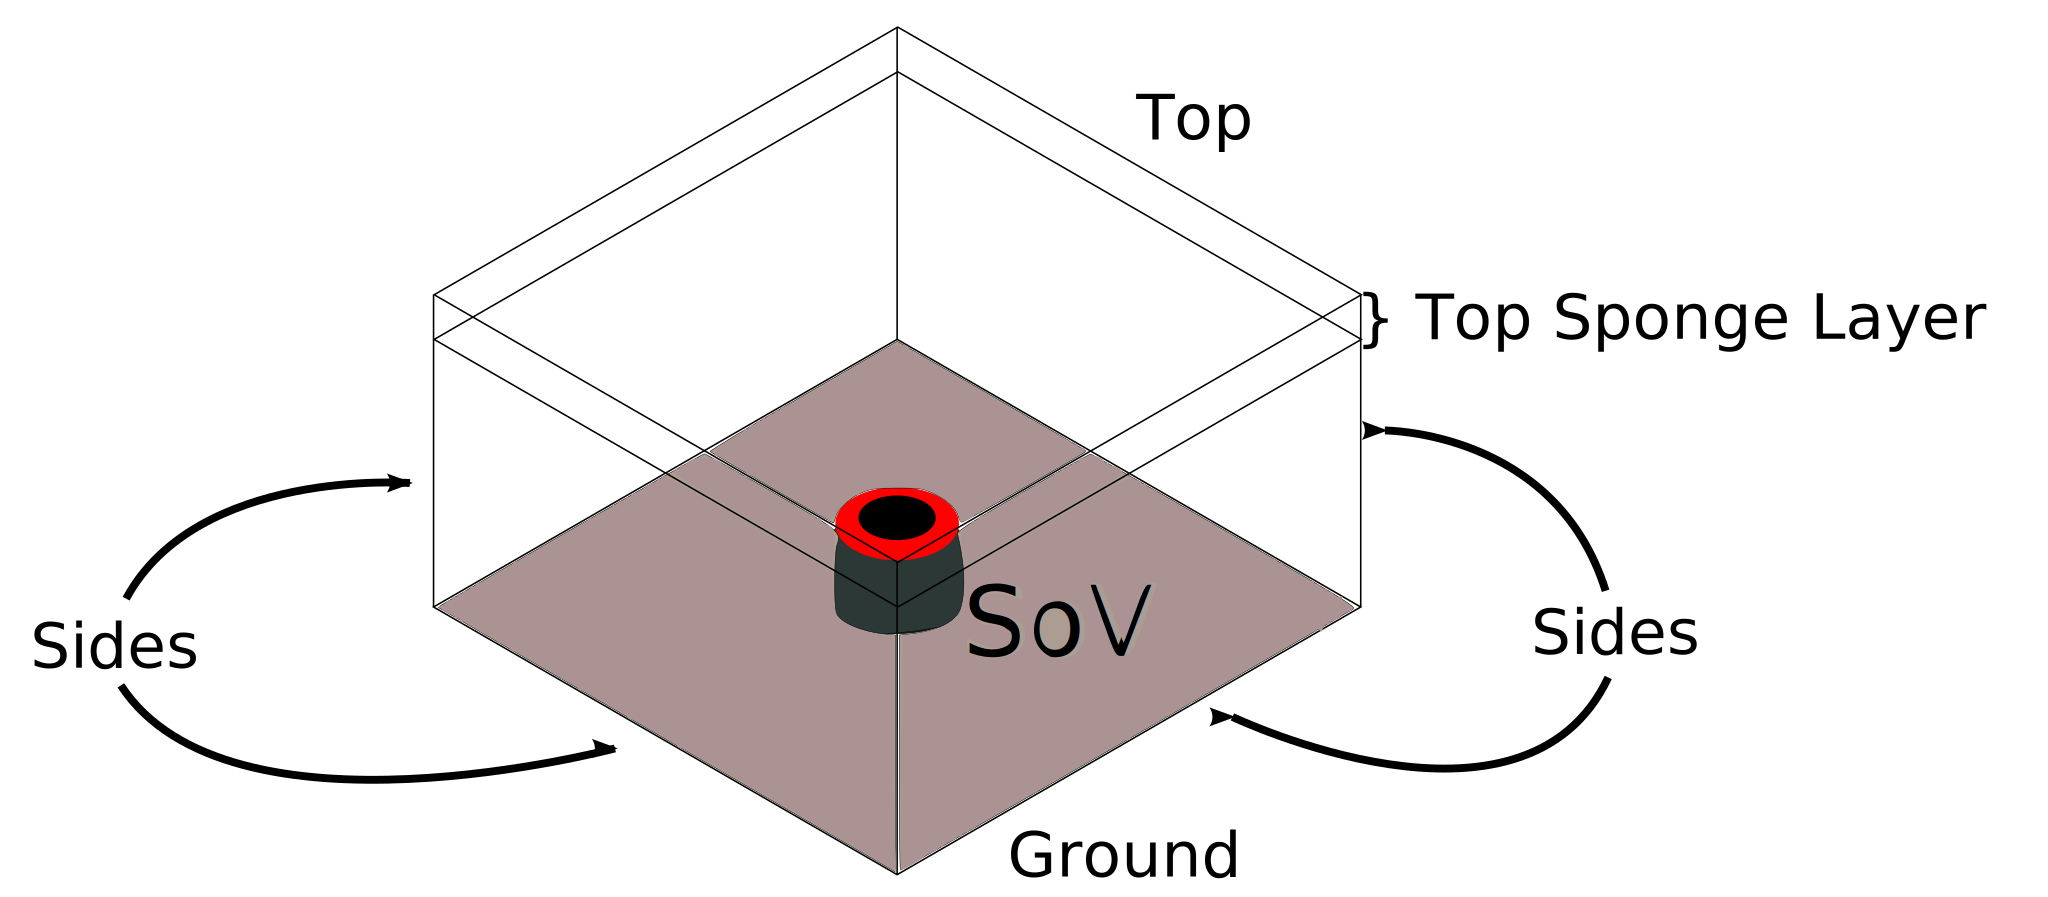
\includegraphics[width=14cm]{figs/thermal_only_3d}
    \caption{Domain for the thermal-only
   scenario. The diagram scale is representative of typical cases. Note
   the SoV apparatus in the center, which provides perspective on the
   extent of the domain with respect to the turning vane diameter. The
   ground, sides and top boundaries are labeled with the discussion the
   precise boundary conditions on each provided in
   Section~\ref{sec:bc}. Notice also the finite thickness, high
   viscosity ``sponge layer'' at the top of the domain.} 
    \label{fig:thermal3d}
  \end{center}
\end{figure}

The boundary for the wind cases is decomposed as,
\begin{equation*}
 \partial \Omega_W = \Gamma_G \, \bigcup \, \Gamma_T \, \bigcup \,
  \Gamma_O \, \bigcup \, \Gamma_I \, \bigcup \, \Gamma_S.  
  \end{equation*}
Where $\Gamma_G$ is the boundary along the ``Ground'',
$\Gamma_T$ the ``Top'' boundary, $\Gamma_S$ the two ``Sides'',
$\Gamma_I$ the inflow boundary, and $\Gamma_O$ the ``Outflow''  
boundary.
The ``wind'' simulation domain is diagrammed in
Figure~\ref{fig:wind3d}, with the boundaries labeled. 
In this wind case (a heated ground with 
an ambient wind), there is a proscribed inlet boundary layer
along the upstream streamwise face ($\Gamma_I$) for both the temperature
and the velocity. The ``Ground'' boundary is identical to
the thermal-only case. The ``Sides'', ``Outflow'' and ``Top'' are all
set to modified Neumann boundary conditions. Note that ``Sponge Layers''
are used on both the outflow and the top. 

\begin{figure}[!htb]
  \begin{center}
   \includegraphics[width=14 cm]{figs/wind_3d}
    \caption{Domain for the wind and thermal scenario. The diagram scale
   is representative of typical cases. Note the SoV apparatus which
   provides perspective on the extent of the domain with respect to the
   turning vane diameter. The ground, sides, inflow, back and top
   boundaries are labeled with the discussion the precise boundary
   conditions on each provided in Section~\ref{sec:bc}. Notice also the
   finite thickness, high viscosity ``sponge layer'' at the top and back
   of the domain.}   
    \label{fig:wind3d}
  \end{center}
\end{figure}

\textbf{Ground Boundary Conditions, $\Gamma_G$} 

For both the wind and thermal-only cases the ground has a fixed
temperature and no-slip velocity boundary conditions. This boundary 
($\Gamma_G$) is modeled with a Dirichlet boundary condition, 
\begin{align}
 {\bf u} &= 0 \quad \text{ on } \Gamma_G \\
 T &= T_g.
\end{align}
Where $\Gamma_G = \{(x,y,0) \subset \partial \Omega \} $. 

%
% http://fenicsproject.org/documentation/dolfin/dev/python/demo/documented/periodic/python/documentation.html 
%
%
\textbf{Periodic Boundary Condition, $\Gamma_P$} 

A periodic boundary condition is used in the thermal only cases, 
for boundaries normal to the x and y directions 
(denoted $\Gamma_{P,x}$ and $\Gamma_{P,y}$, respectively). In these
cases the state variables  
are contrained to have the same value on the opposite faces of the domain, 
for instance in the streamwise direction the boundary conditions are, 
\begin{align}
 {\bf u}(-L_x,y,z) &= {\bf u}(L_x,y,z) \quad \text{ on } \Gamma_{P,x} \\
 T(-L_x,y,z) &= T(L_x,y,z)
\end{align}
and in the spanwise direction,
\begin{align}
 {\bf u}(x,-L_y,z) &= {\bf u}(x,L_y,z) \quad \text{ on } \Gamma_{P,y} \\
 T(x,-L_y,z) &= T(x,L_y,z). 
\end{align}
Where $\Gamma_{P,x} = \{(-L_x,y,z) \, \bigcup \, (L_x,y,z) \subset \partial
\Omega \}$  
and $\Gamma_{P,y} = \{(x,-L_y,z) \, \bigcup \, (x,L_y,z) \subset \partial
\Omega \}$. 

\textbf{Inflow Boundary Condition, $\Gamma_I$} 

On the inflow boundary $(\Gamma_I$), dirichlet conditions are used for
both velocity and temperature. The boundary-normal, or streamwise
component is a function of the surface normal coordinate (z),
representing a boundary layer below a uniform velocity, U.
The common 7\textsuperscript{th} power model of a turbulent boundary
layer is used,    
\begin{equation*}
  u_{\text{in}}(z) = U \text{ min }\left(\left(\frac{z}{\delta}\right)^7,1\right),
  \label{eq:bl_u}
\end{equation*}
where $\delta$, the boundary layer thickness, is set based on data
measured by our experimental partners in the field. 
The thermal boundary layer is assumed to have a similar boundary layer,
but, as observed in real atmospheric flows, there remains a vertical
temperature gradient outside the thin boundary layer. 
The thermal inflow has the form,
\begin{equation*}
  T_{\text{in}}(z) = \Delta T \left(1- \text{ min
			}\left(\left(\frac{z}{\delta}\right)^7,1\right)\right)
  + T_0 - \beta z.  
  \label{eq:bl_t}
\end{equation*}
% 335+18*tanh(-z/0.1)-z*2/3
Based on results in the literature, $\beta = 2/3$ Kelvin per 
meter\cite{Blocken2007238}.
This inflow boundary is at the surface $x=-L_x$.

\textbf{Mixed inflow/outflow Boundary Conditions on $\Gamma_T$,
$\Gamma_S$ and $\Gamma_B$}  

At outflow boundaries, a homogeneous Neumann condition is
appropriate\cite{Rannacher2000}, 
\begin{align}
  \frac{\partial u}{\partial n}\bigg|_{\Gamma_T} = 0, \\
  \frac{\partial T}{\partial n}\bigg|_{\Gamma_T} = 0.
\end{align}
However, for the cases in this study, a modified Neumann condition is
necessary due to the possibility that there will be an inflow on these
boundaries. 
For example, in the region above the vanes, the concentrated hot plume is
lifted by buoyancy upward and out of the simulation domain. However, the
radial inflow towards the apparatus is drawn in by large scale
convection cells larger than the system diameter. Thus, our boundary
conditions must permit inflow along the areas above and external to the
vanes, while simultaneously permitting outflow in the area above the vanes. 

% Roy Stogner: Okay, so this DDN is basically no-traction when there's 
% outflow and Tn=v when there's inflow?  We have no-traction for v*n, 
% no-traction for anything else when there's outflow, and Dirichlet
% v.cross.n = 0 when there's inflow. 

To accomplish this, the boundary condition is,
\begin{align}
  \frac{\partial u_n}{\partial n}\bigg|_{\Gamma_T} = 0 \\
  \text{if } (w<0) \text{ then}& \begin{cases}
    u_t = 0,\\
    T = T_{\text{in}}
  \end{cases} \\
  \text{ else}& \begin{cases}
    \frac{\partial u_t}{\partial n}\bigg|_{\Gamma_T} = 0, \\  
    \frac{\partial T}{\partial n}\bigg|_{\Gamma_T} = 0
  \end{cases}
\end{align}
where $u_n$ and $u_t$ are normal and tangential components of the velocity, 
respectively. This boundary condition is applied on the top boundary
$\Gamma_T$ ($z=L_z$) and downstream side boundary  $\Gamma_B$ in the
wind case. This mixed boundary condition appears to be a unique
implementation of a modified Neumann condition condition, which has been 
demonstrated previously in other
instances~\cite{braack2014directional,feistauer2006non}. In particular,
the well-posedness of this general class of boundary condition is
treated in \cite{bruneau1996new}.  

\textbf{Sponge Layer} 

Finally, a finite thickness ``sponge layer'' is used in the region adjacent 
to the mixed inflow/outflow boundaries $\Gamma_T$ and $\Gamma_B$.
These regions are referred to by many names in the
literature\cite{doi:10.1146/annurev.fluid.36.050802.121930}, such as
absorbing layers, fringe regions, buffer zones, sponges,
etc. 
This layer artificially increases the momentum diffusivity by
a factor of ten over the nominal value. This was designed to stabilize
the modified Neumann boundary conditions which can exhibit an instability
when there is a compact jet of fluid leaving the domain. 
These small outflows would create small high velocity inflows, and the
feedback loop would result in instabilities and numerical
blow-up. 
% Mindful of the fact that the character of solution not
% important in this region, and that our physical interest remains focused
% on the region inside and in immediate proximity to the vanes, we
% introduced a higher diffusivity ``sponge'' region that would diffuse the
% high velocity exiting jets sufficiently to prevent numerically
% un-physical behavior. 
Use of this stabilizing sponge layer is justified because we are not
interested in the flow in this region. 
No results are quoted from this ``sacrificial''
region, as it is not considered physically meaningful. The top sponge
layer in both the wind and thermal-only cases are half a
system diameter $(L_z/D = 1/2)$ thick. For the wind cases, the
downstream sponge layer is also half a system diameter $(L_x/D
= 1/2)$ thick.  

%\todo{expand this? how thick did it need to be?}
